\section{Evidence strategy: complementary studies, not pooled replication}
The research questions require different tests. A fixed-topology study isolates
objective-conditioned parameter selection. Structural cases test whether novel
source, protocols and routes actually reach native activities. Gradient pilots
test derivative meaning and subsequent native forwards. The latest matched
study compares local-designer packages and stronger references on a common
source. Table~\ref{tab:integrated-studies} summarizes these roles.

\begin{table}[t]\centering\small
\caption{Evidence families retained in the integrated argument. Counts are
within-study budgets, not additive independent replications. Historical
source/model/feedback differences prevent pooling method rankings.}
\label{tab:integrated-studies}
\begin{tabular}{@{}>{\raggedright\arraybackslash}p{.19\linewidth}>{\raggedright\arraybackslash}p{.21\linewidth}>{\raggedright\arraybackslash}p{.25\linewidth}>{\raggedright\arraybackslash}p{.25\linewidth}@{}}
\toprule
Family & Design/author & Native evidence & Question addressed \\
\midrule
Parameter study & Eight fixed-topology settings; adaptive random search & 45 logical development rows; 15 sealed evaluation runs & Can objective changes select different systems and profiles? \\
Structural cases V8/V12 & External source/protocol/graph author & Eight/six two-year worlds & Do new mechanisms, routes and plan processes execute? \\
Nested case V13 & External vocabulary + conditional LR + redesign & Eight worlds; 592 fresh replies & Can inner updates and outer source changes share a native loop? \\
Gradient cases V9--V11 & Response representation, local refinement, score/control estimator & Coupled paths and eight reset worlds, separately bound & Does backward mean fidelity, a native-tested update or superiority? \\
Matched study V2 & Local 35B designer and uniform numeric control & 120 attempts; 90 selection-fixed evaluations & What is achieved under matched permitted freedoms and stronger references? \\
\bottomrule
\end{tabular}\end{table}

Across native case studies, five original researchers and fixed Qwen3-8B
weights retain language decisions, literature grounding, projects and papers.
Most cases use two years and development seed 42; the older parameter study
uses four-year worlds and a different source/seeding protocol. A common seed
does not force equal fresh LLM realizations. We distinguish reset worlds,
common-prefix-coupled forwards, conditional IID design draws and genuinely
unused evaluation conditions. No new inference is introduced by this synthesis.

\section{Objective-conditioned parameter optimization}
\label{sec:parameter}
\subsection{Design and sealed evaluation}
The first study varies eight institutional settings within one fixed topology:
acceptance rate, funding application cost, funding slot fraction, resubmission
cost, review policy, reviewer capacity, reviewer matching and reviews per paper.
The simulator, adaptive-random-search rule, five-candidate budget and development
seeds 601/607/617 are held fixed while the optimized LossSpec changes.
For valid run $ r $, the losses are
\begin{align}
 \ell_r^{\rm part}&=1-a_r+0.05b_r,&
 \ell_r^{\rm topic}&=-h_r,&
 \ell_r^{\rm burden}&=b_r,
\end{align}
where $ a_r $ is active-researcher fraction, $ b_r $ review burden per active
researcher and $ h_r $ topic entropy. Each arm minimizes the development mean
plus $0.25$ population standard deviations over its three seeds. Entropy is
not truth, and burden can fall by suppressing evaluation. These deliberately
narrow proxies stress the objective-to-system map.

All 45 logical design--seed rows terminate: 30 complete and 15 fail at the declared
reviewer-capacity boundary, retaining null loss. Twenty-nine development rows
are physically executed and 16 logical rows adopt byte-identical initial
trajectories under the study's provenance contract. Thus 45 logical rows are
not 45 fresh native worlds. All winners are sealed before a common evaluation
on unused seeds 701/709/719/727/733; all 15 arm-labelled runs complete.

\subsection{Different objectives, two actual designs}
Participation/review selects proposal 2 with development loss 0.321846. Topic
and burden select proposal 1, with losses $-1.696931$ and $1.668963$. In the
topic arm proposals 1/2 tie, so the predeclared earliest rule selects 1. Only
participation has multiple valid adaptive proposals beyond the initial pair;
later topic/burden proposals fail technical validity. The paths show an
executable own-observation loop, not rich or repeatable path divergence.

The selected participation design has acceptance rate 0.4968, capacity 8,
topic-based matching and three reviews per paper. Topic/burden share a design
with rate 0.1132, capacity 2, random matching and four reviews per paper.
Three objective labels therefore produce two designs, not three institutions.
Full settings appear in Appendix~\ref{app:parameter}.

\begin{figure}[t]\centering
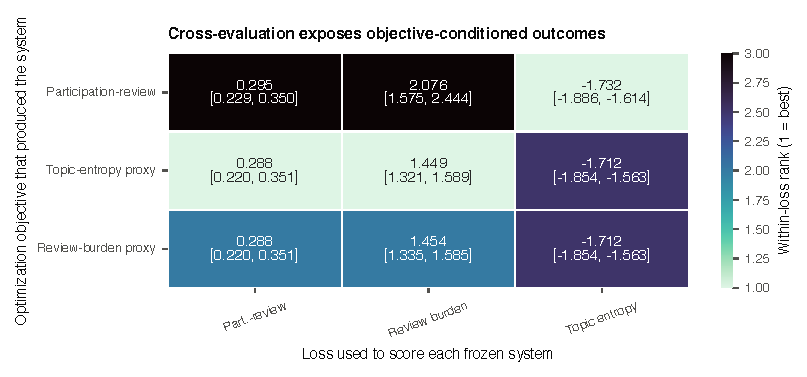
\includegraphics[width=\linewidth]{generated/metric-conditioned/figures/metric-conditioned-cross-evaluation.pdf}
\caption{\textbf{Historical parameter study: sealed-system cross-evaluation.}
Numbers are each complete LossSpec aggregate with the study's exact-bootstrap
percentile intervals over five unused seeds; color ranks within a loss only.
Topic and burden rows encode the same design but separate stochastic evaluations.
All nine paired-contrast intervals include zero. Descriptive ordering is not
stable superiority or evidence that every objective discovers a distinct system.}
\label{fig:integrated-parameter}
\end{figure}

On unused conditions, the participation-selected design has aggregate losses
0.295 on participation, 2.076 on burden and $-1.732$ on topic. The duplicated
topic/burden design has approximately 0.288, 1.449--1.454 and $-1.712$.
Ordering changes with the scoring loss, but every one of the nine paired
95\% intervals includes zero. The apparent rank reversal is descriptive.
The selected design is not necessarily best under its own unused-condition loss.

Operational differences are clearer than normative conclusions. The
participation-selected design averages 11.6 accepted papers and full review
coverage, versus 4.0 and approximately 0.55 for the other design. It also has
higher burden, approximately 1.959 versus 1.415--1.421. Activity fractions 0.82
versus 0.80 and topic entropies 1.771 versus 1.750 remain uncertain at five seeds.
This is not a welfare ranking, optimizer comparison or structural-search result.

\section{Executing institutions beyond fixed parameter menus}
\label{sec:structural}
\subsection{A new planning and delayed-feedback route}
The external-author V8 case permits source, intermediate protocols, node
addition/removal, wiring and activity processes. Two objectives use
$T=-A$ and $U=3.25A-Q+0.05R$, where $A$ counts accepted native decisions,
$Q$ sums original reviewer-score means on accepted decisions, and $R$ counts
review records. Authored final scores do not create $Q$. Each objective has
two generations and two conditional-IID draws per generation.

All eight native worlds complete with 734 fresh Qwen replies. The developer
seed has 19 nodes/27 edges; evaluated graphs have 16--18 nodes/22--24 edges.
Throughput losses are $[-9,-9,-10,-10]$; utility losses are
$[0, 0, 0.4833, 0.4833]$. All outcomes are retained in
Appendix~\ref{app:structural}; these same-seed development worlds are not
an unused-condition causal comparison.

Throughput redesign replaces hash-selected plan eligibility with actual
deadline inspection and annual amendments. In the first revised world,
a researcher whose project would finish in year 2 has a real amended plan
finishing in year 1 and an actual year 1 accepted-paper record. Five rather
than four year 1 submissions/acceptances are recorded. A newly wired publication
receipt route delivers earlier paper identities to the year 2 planning node,
and resulting focus text reaches actual researcher requests.

Timing limits the mechanism claim. The extra year 1 acceptance occurs before
any prior publication receipt exists; it cannot be attributed to that delayed
feedback. Source, scope, focus and wiring change jointly, without component
ablation. What is established is an exercised plan/record/information path,
not the independent benefit of the added feedback loop.

The utility revision adds review-digest feedback and restores review. It accepts
one paper with mean score $11/3$ after 18 reviews, yielding
$3.25-11/3+0.05(18)=0.4833$. The initial no-review/no-acceptance observations
remain better at 0. A new mechanism can be technically real and worse under the
declared objective. No quality or participation veto reverses that result.

\subsection{An executed new mechanism that is not retained}
The V12 case gives each objective three own-history source redesigns. All six
worlds complete with 565 fresh replies. Throughput installs a production office,
annual scheduler and all-accept decision source, producing 10 native plan
amendments and 10 acceptances per world. Later generations retain the exact
first institution; the loss path $[-10,-10,-10]$ is not repeated invention.

Utility begins with an evidence office and an original-review threshold above
3.25. Its G1 introduces a genuinely executed milestone-clinic node, typed
amendment transport and two wires, and changes evidence-topic matching. It
shortens one project and extends another to a two-year cycle; it is not simply
a universal acceleration rule. The native world completes, but utility worsens
from $-1/6$ to 0 with 15 reviews. G2 returns to the G0 incumbent, giving
$[-1/6, 0,-1/6]$.

The G2 parent is the best G0, not chronological G1. A zero parent diff therefore
correctly records retention, while the chronology still exposes the unsuccessful
clinic. This case matters because it demonstrates actual mechanism/wiring
freedom without selecting only successful-looking revisions. It does not
establish which simultaneous edit caused the changed loss.

\section{Nested free design and conditional distribution updating}
\label{sec:nested}
\subsection{One loop, two levels of freedom}
The V13 case combines an externally authored institutional vocabulary with
one within-vocabulary likelihood-ratio update and a fresh native followup.
Each of two losses, $T=-A$ and $E=-Q+0.5R$, receives exactly four scheduled
worlds: two IID G0 design draws, one draw from saved updated G0 weights and
one free G1 source redesign. All eight complete with 592 fresh scientist replies
and no response reuse. Every world resets development seed 42. The external
Codex author identity is self-reported, not authenticated local-Qwen authorship.

For two draws, the implemented LOO estimate is
\begin{equation}
 \widehat g=\tfrac 12\left[(L_0-L_1)s_0+(L_1-L_0)s_1\right],\qquad
 s_i=\nabla_\theta\log q_\theta(d_i\mid V),\quad
 \theta^+=\theta-0.1\widehat g.
\end{equation}
The followup uses exactly that saved vocabulary/distribution and performs no
extra update. G1 then sees only its own three preceding observations, source,
failures and saved update; it may change algorithms or support. Removing all
coordinates explicitly creates a point mass rather than silently reusing old
weights. A completed update is not itself evidence of lower expected loss.

\begin{table}[t]\centering\small
\caption{\textbf{All nested-study outcomes.} These are same-development-seed
worlds, not independent scientific seeds. $Q$ is original peer evidence.
The post-update draw is not omitted when it worsens.}
\label{tab:integrated-nested}
\begin{tabular}{llrrrrr}\toprule
Optimized loss & Stage & $A$ & $Q$ & $R$ & $T$ & $E$\\\midrule
Throughput & G0 draw 1 &7&0&0&-7&0\\
 & G0 draw 2 &7&0&0&-7&0\\
 & Updated G0 &6&0&0&-6&0\\
 & Free G1 &10&0&0&-10&0\\\addlinespace
Reviewed production & G0 draw 1 &6&20&6&-6&-17\\
 & G0 draw 2 &6&18.5&12&-6&-12.5\\
 & Updated G0 &6&12&4&-6&-10\\
 & Free G1 &6&21&6&-6&-18\\\bottomrule
\end{tabular}\end{table}

\subsection{Distribution changes and native-tested redesign}
Equal initial throughput losses give zero centered advantages and unchanged
Gaussian mean. Its next native draw has loss $-6$, worse than $-7$; it is not
reported as a successful gradient proposal. Reviewed-production losses
$[-17,-12.5]$ produce a nonzero update: the coverage latent mean changes from
1.5 to 1.671086 and reviewer-count logits from $(-1, 1,-1)$ to
$(-1, 1.225,-1.225)$. The next native draw has loss $-10$, also worse than its
prior best. Neither sample demonstrates expected improvement or estimator
superiority, nor does one worsening sample refute the score identity.

The later throughput source revision replaces mixed-cycle hashing with
universal annual scheduling while preserving native topic, focus and reason
fields. The zero-review dispatcher and compatible all-accept rule remain.
Observed loss improves from $-7$ to $-10$. Reviewed-production G1 replaces the
coverage lottery with full coverage and one eligible reviewer per paper, ranked
by its own historical scores. A read-only join rechecks the 22 original review
records used in that ranking, including shrinkage toward a pooled mean.
Task identities change, but actual Qwen reviews and the original parser still
determine $Q$. Its observed loss improves from $-17$ to $-18$.

\begin{figure}[p]\centering
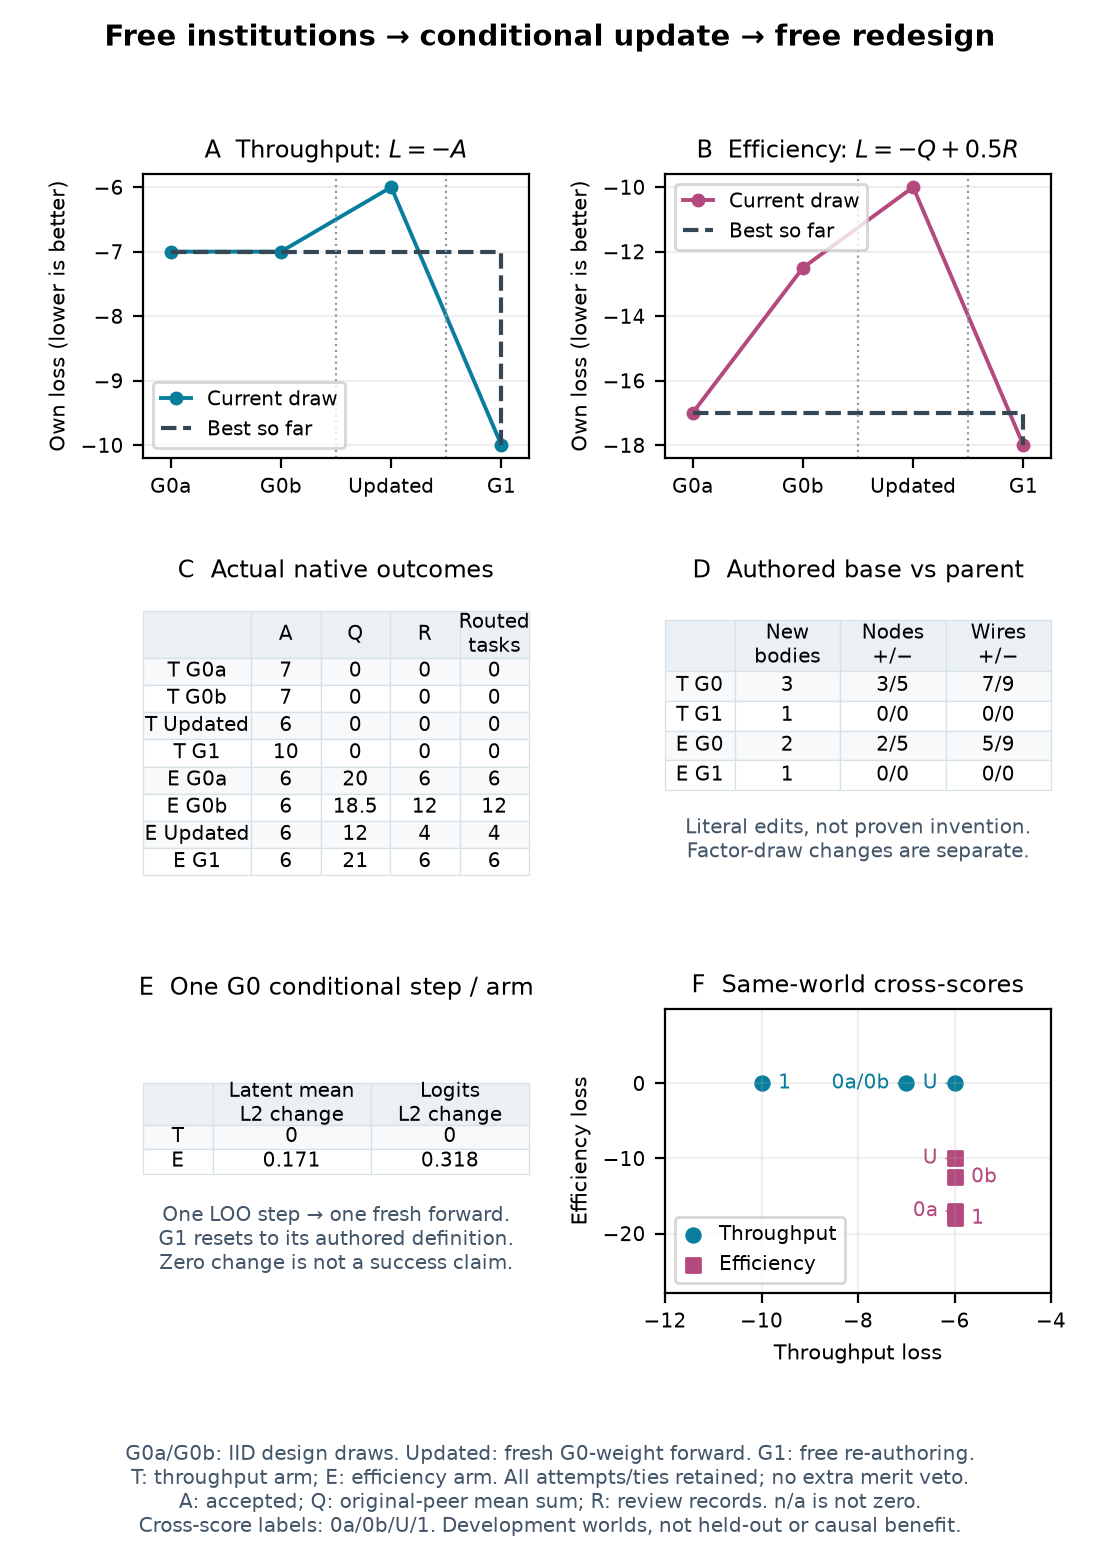
\includegraphics[width=\linewidth,height=.79\textheight,keepaspectratio]{figures/native-nested-search-v13-a1.png}
\caption{\textbf{Complete native nested-design paths.} Current observations,
best-so-far, actual $A/Q/R$, literal changes and conditional updates remain
separate. Both gradient followups are worse than their prior best; both later
external code revisions improve their observed first best. ``Efficiency'' here
means the illustrative $E$ proxy, not scientific efficiency or welfare.
Cross-scores reuse the same checkpoints; they are not held-out evidence.}
\label{fig:integrated-nested}
\end{figure}

Initial free vocabularies already differ from their common parent; G1 changes
one source body in each arm while graph sizes remain 17/25 and 16/23. Thus these
are algorithmic edits without new G1 topology. Actual source/plan/wire/task
receipts verify 40 source executions, 16 complete-plan effects, 16 routing events
and 28 review records. These establish exercised native effects, not a causal
decomposition of the gain. Favorable-reviewer selection exposes a proxy-seeking
route, not improved scientific evaluation. No hidden merit veto removes it.

\section{What native gradient experiments establish}
\label{sec:gradient-evidence}
\subsection{A fitted response representation can fail unused conditions}
The V9 case varies a charter's evidence weight $\theta $, paired with originality
weight $1-\theta $. The charter enters actual year 2 reviewer requests after the
pre-intervention native history. Scientist weights and the original integer
review parser stay fixed. The loss is $U=3.25A-Q+0.05R$.

Three calibration endpoints $\theta=(0.2, 0.5, 0.8)$ fit per-review raw-response
operators. Calibration-loss RMSE chooses a declared relaxation temperature;
the operator and proposal are frozen before unused coordinates 0.35/0.65 are
read. At the center, a clipped negative-gradient step is followed by a native
execution, even if it is a no-op. These are unused coordinates within one
development history, not unused world seeds.

Six forwards use a verified 53-reply common prefix and then 31 fresh replies each:
504 logical responses comprise 318 replays and 186 new calls. They are not six
independent societies. The fitted temperature 0.01 achieves calibration-loss
RMSE$1.16\times 10^{-5}$, yet its center derivative is only
$1.15\times 10^{-15}$. The prescribed proposal is the unchanged 0.5, with native
loss 0.9. The known lower calibration endpoint at 0.8 is not substituted for it.

At unused 0.65, predicted loss is approximately 0.8168 but native loss is 0.9.
Across $0.35\to 0.65$, native change is zero, the response-aware representation
predicts $-0.08395$, and the frozen-response baseline predicts zero. The
representation therefore fails the declared finite-path check and does not
improve prediction here. This is a substantive boundary result: native
ingress, identity joins, loss accounting and backward all execute, while
fidelity and a useful native update remain unestablished.

\subsection{Different update paths, the same observed incumbent}
V10 compares represented gradients with local derivative-free interval
refinement, charging both three shared historical calibration evaluations
and three fresh attempts. The current coordinate starts at 0.5, but both already
know the historical incumbent 0.8 with loss $49/60\approx 0.8167$.
The gradient method has raw responses/traces; the black-box method receives
coordinates/scalars only. Equal evaluation count is not equal information.

\begin{table}[t]\centering\small
\caption{Native-tested moving paths. Both methods know the better historical
point before these proposals. A moving current iterate is not a new best.}
\label{tab:integrated-method-paths}
\begin{tabular}{lrrrr}\toprule
Method & $\theta_1$ & $\theta_2$ & $\theta_3$ & Native loss sequence\\\midrule
Represented gradient & .6000 & .6488 & .7488 & $(.9000,.8167,.8167)$\\
Black-box refinement & .6500 & .7250 & .7625 & $(.9000,.8167,.8167)$\\\bottomrule
\end{tabular}\end{table}

All six fresh attempts complete, generating 186 new replies after their shared
prefixes. The represented derivatives $(-.24092,-.09762,-1.24626)$ yield different
coordinates, but native loss sequences coincide and neither beats the already
known incumbent. This demonstrates real proposed updates and measured paths,
not a gradient advantage. Appendix~\ref{app:gradient} retains the temperature
diagnosis explaining why calibration fit alone was insufficient.

\subsection{Conditional LR and corrected controls reach native execution}
V11 uses explicit mean/minimum reviewer aggregation and a bounded cutoff
driven by a Gaussian latent in one authored vocabulary. Eight fresh worlds
compare a derivative-free feedback heuristic with score updating. Both arms
observe $[0.7833333, 1.2, 1.2, 1.2]$ and retain their first incumbent; 742 fresh
replies are recorded. Prior-frozen controls implement
Eq.~\eqref{eq:integrated-control}, but the final control update is saved after
the last measured batch, not tested again within that budget.

A separately budgeted two-world V12 followup evaluates that exact saved
distribution: minimum aggregation at cutoff 3.549508 gives $A=Q=0,R=21,U=1.05$;
mean aggregation at 3.080488 gives $A=2,Q=7,R=21,U=0.55$. These 180 fresh replies
close the missing-forward question. The two outcomes do not establish lower
expected loss, lower variance or a concurrent advantage over V11's historical
outcomes. The distinction between a computed derivative, a saved proposal
and a native-tested distribution is preserved across all these cases.
\FloatBarrier
